\chapter{Computing Sensitivity in Practice}

\begin{flushright}
\textit{A derivative is useful only if you can compute it honestly.}
\end{flushright}

\bigskip

You have inherited a model from a collaborator.
It is 500 lines of MATLAB code, produces reasonable epidemic
projections, and has 11 parameters.
Your collaborator has moved to another institution.
The code runs correctly, but it uses conditional statements,
lookup tables, and an internal adaptive ODE solver;
none of which can be differentiated analytically.
Your funding agency wants to know which parameters matter
before committing to a three-year field measurement campaign.

How do you compute sensitivity indices for a model you cannot
differentiate?

The answer is finite differences, and this chapter shows exactly
how to do it, including how to avoid the mistakes that produce
wrong results.

%%------------------------------------------------------------
\section{The Sensitivity Jacobian}
\label{sec:jacobiansec}
%%------------------------------------------------------------

Chapter~2 computed sensitivity indices one parameter at a time.
For a model with $n_p$~\POIs and $n_q$~\QOIs,
the complete local SA is captured by an $n_q \times n_p$ matrix;
one entry per \POI--\QOI pair.

\begin{definition}[Sensitivity Jacobian]\index{sensitivity Jacobian}
\label{def:SJacobian}
Let $\vec{q} = (q_1, \ldots, q_{n_q})$ denote the vector of \QOIs
and $\vec{p} = (p_1, \ldots, p_{n_p})$ denote the vector of \POIs.
The \textbf{normalized sensitivity Jacobian}\index{sensitivity Jacobian!normalized} is the
$n_q \times n_p$ matrix $\mathbf{S}$ with entries
\begin{equation}
  S_{ki} = \SI{p_i}{q_k} = \frac{p_i}{q_k}\,\pd{q_k}{p_i}.
  \label{eq:SJacobian}
\end{equation}
\end{definition}

For the SIR model with \POIs $\{k, \beta, \tau, \mu\}$
(contact rate, transmission probability, mean infectious period,
mortality rate) and \QOIs $\{S(T), I(T), R(T)\}$ (the three
compartment sizes at time $T$), the sensitivity Jacobian is a
$3 \times 4$ matrix of twelve numbers.
Each number answers one specific "What if?" question:
how much does compartment $i$ change if \POI $j$ changes by $1\%$?

The tornado plots in Chapter~2 displayed single rows or columns
of this matrix. The full matrix captures all
\POI--\QOI relationships simultaneously.

Computing this matrix efficiently, in both time and accuracy;
is the central computational challenge of sensitivity analysis.

A common initial reaction is to treat the sensitivity Jacobian as
nothing more than a collection of individual SI calculations;
as if the matrix label were just a convenient way to organize numbers
that are computed independently. It is more than that.
The Jacobian has structure: its columns can be computed in parallel,
many methods share a single baseline evaluation, and the adjoint
method (Chapters~5 and 6) exploits the matrix structure to recover
all columns at once from a single backward solve. Understanding the
Jacobian as a matrix, not just a table, is what makes efficient SA possible.

\begin{selfcheck}
A climate model has $n_p = 30$ \POIs and $n_q = 8$ \QOIs.
How many individual sensitivity indices does the full SA require?
If you had to compute each one separately, how many model
evaluations would a naive brute-force approach require?
\end{selfcheck}
\begin{scAnswer}
$30 \times 8 = 240$ sensitivity indices. A naive approach, perturb
one \POI at a time, re-run the model, compute the difference;
requires $30 + 1 = 31$ model evaluations for all \POIs simultaneously
if only first-order (forward) differences are used, or
$2 \times 30 + 1 = 61$ for centered differences.
The key: you do not need one evaluation per SI entry. You need one
evaluation per \POI (plus one baseline), and then each evaluation
contributes an entire column of the Jacobian.
\end{scAnswer}

%%------------------------------------------------------------
\section{Finite Difference Formulas}
\label{sec:finitediff}
%%------------------------------------------------------------

A finite difference approximates the partial derivative
$\partial q/\partial p_i$ by computing how the \QOI changes when
$p_i$ alone is shifted by a small but finite amount $h$.
Three approximations are in common use, differing in accuracy and cost.

\subsection{Forward Difference}

The simplest approximation uses one additional model evaluation:
\begin{equation}
  \pd{q}{p_i} \approx \frac{q(p^* + h\vec{e}_i) - q(p^*)}{h},
  \label{eq:FD1}
\end{equation}
where $\vec{e}_i$ is the unit vector in the $p_i$ direction and
$p^*$ is the nominal parameter vector.
This is a first-order approximation: the error is $O(h)$,
meaning that halving $h$ approximately halves the error.

\subsection{Centered Difference}

Using one evaluation on each side of the nominal value gives
a second-order approximation:
\begin{equation}
  \pd{q}{p_i} \approx \frac{q(p^* + h\vec{e}_i) - q(p^* - h\vec{e}_i)}{2h}.
  \label{eq:FD2}
\end{equation}
The error is $O(h^2)$: halving $h$ reduces the error by a factor of four.
For the same step size, centered differences are substantially more
accurate than forward differences.

\subsection{Fourth-Order Formula (Rarely Used in Practice)}

When exceptionally high accuracy is required and model evaluations
are inexpensive, one can eliminate the leading-order error term
by combining four evaluations at two step sizes:
\begin{equation}
  \pd{q}{p_i} \approx
    \frac{-q(p^*+2h\vec{e}_i) + 8q(p^*+h\vec{e}_i)
          - 8q(p^*-h\vec{e}_i) + q(p^*-2h\vec{e}_i)}{12h}.
  \label{eq:FD4}
\end{equation}
The error is $O(h^4)$: halving $h$ reduces the error by a factor of
sixteen. This requires four evaluations per \POI rather than two.
In the applied SA literature this formula is uncommon; the
centered difference~\eqref{eq:FD2} is the standard workhorse.
Knowing which formula to use and what step size to choose are the
practical skills taken up next.

\subsection{Practical Workflow: Step-Size Selection by Error Estimation}

In practice, the centered difference~\eqref{eq:FD2} is the
default choice. The forward difference~\eqref{eq:FD1} plays a
secondary role not as a first approximation in its own right,
but as a cheap error estimator: because it requires only the
already-computed baseline $q(p^*)$ and the one-sided perturbed
evaluation $q(p^*+h\vec{e}_i)$, no extra model runs are needed.
The difference between the two approximations at the same $h$,
\begin{equation}
  \text{estimated error} \approx
  \left|
    \frac{q(p^*+h\vec{e}_i) - q(p^*)}{h}
    -
    \frac{q(p^*+h\vec{e}_i) - q(p^*-h\vec{e}_i)}{2h}
  \right|,
  \label{eq:FDerror}
\end{equation}
provides a practical error indicator. If this indicator is large
relative to the desired precision, the analyst reduces $h$ (or
increases ODE solver tolerances) and repeats until the error is
acceptable. This adaptive strategy is more reliable in practice
than deriving a theoretical optimal $h$ from
equations~\eqref{eq:hopt_fwd}--\eqref{eq:hopt_cen}, because
those formulas depend on unknown higher-order derivatives of the
model output.

A complementary check uses the backward difference
$[q(p^*) - q(p^*-h\vec{e}_i)]/h$ as a second one-sided estimate.
Comparing both one-sided approximations with the centered result
gives two independent error indicators, and agreement among all
three signals that $h$ lies in the reliable range.

\subsection{Cost Comparison}

Table~\ref{tab:FDcost} summarizes the cost of computing the
complete sensitivity Jacobian by each method.

\begin{table}[htb]
\centering
\begin{tabular}{lccl}
\toprule
Method & Model evaluations & Error order & Best when \\
\midrule
Forward difference   & $n_p + 1$       & $O(h)$   & Error check only; not standalone \\
Centered difference  & $2n_p + 1$      & $O(h^2)$ & Standard choice \\
Fourth-order FD      & $4n_p + 1$      & $O(h^4)$ & Rare; cheap evaluations only \\
Analytic FSE (Ch.~4) & $n_p$ lin.\ solves & Exact  & Differentiable model \\
Adjoint (Ch.~5--6)  & 2 solves        & Exact    & Many \POIs, few \QOIs \\
\bottomrule
\end{tabular}
\caption{Cost of computing the complete sensitivity Jacobian by
         different methods, for a model with $n_p$~\POIs and
         $n_q$~\QOIs. The number of model evaluations does
         \emph{not} depend on $n_q$: each evaluation contributes
         an entire column of the $n_q \times n_p$ Jacobian simultaneously.
         Adding more \QOIs is free --- the cost scales with
         the number of \POIs $n_p$, not with the size of the output.
         The finite-difference counts assume a single
         baseline evaluation is reused across all \POIs.}
\label{tab:FDcost}
\end{table}

For the SIR model with $n_p = 4$ parameters and $n_q = 3$ state
variables, centered differences require
$2 \times 4 + 1 = 9$ model evaluations.
If each takes 1~second, the full SA takes 9~seconds.

For the malaria model of Chitnis, Hyman \& Cushing~\cite{chitnis2008determining}
with $n_p = 17$ parameters and $n_q = 7$ state variables,
centered differences require $2 \times 17 + 1 = 35$ evaluations.
If each takes 1~minute: approximately 35~minutes.
If each takes 1~hour: approximately 35~hours.

For a climate model with $n_p = 500$ parameters and
model runs taking 6~hours each, centered differences require
$2 \times 500 + 1 = 1001$ evaluations, at 6~hours each,
that is approximately 250~days of computation.
This is why Chapter~6 introduces the adjoint method, which
reduces the cost to 2 solves regardless of $n_p$.

\unifyingidea{1} Every entry of the sensitivity Jacobian is a
normalized derivative: an instance of Unifying Idea~1 from
Chapter~1. The finite-difference formulas in this chapter
compute those derivatives numerically, for any model that
can be evaluated, whether or not it can be differentiated
analytically.

\begin{selfcheck}
For a model with $n_p = 20$ \POIs and $n_q = 5$ \QOIs,
how many model evaluations does the centered-difference Jacobian require?
(Remember: adding more \QOIs is free --- each evaluation contributes
an entire column of the Jacobian.)
If each evaluation takes 45~seconds, how long does the complete SA take?
At what value of $n_p$ would centered differences take more than 24~hours,
assuming each evaluation takes 2~minutes?
\end{selfcheck}
\begin{scAnswer}
$2 \times 20 + 1 = 41$ evaluations, regardless of $n_q = 5$;
$41 \times 45 = 1{,}845$~seconds $\approx 31$~minutes.

For 24~hours $= 1{,}440$~minutes with 2-minute evaluations:
$2n_p + 1 \leq 720$ gives $n_p \leq 359$, so for $n_p \geq 360$,
centered differences take more than 24~hours.
\end{scAnswer}

%%------------------------------------------------------------
\section{Step Size Selection --- The U-Curve}
\label{sec:ucurve}
%%------------------------------------------------------------

The step size $h$ controls a fundamental accuracy tradeoff.
There is an optimal value: too large and the approximation
misses the local curvature; too small and the computer's
limited numerical precision destroys the result.

\subsection{Two Sources of Error}

\textbf{Truncation error}\index{truncation error} arises because finite differences
are Taylor-series approximations. For the centered difference:
\begin{equation}
  \frac{q(p+h) - q(p-h)}{2h}
  = q'(p) + \underbrace{\frac{h^2}{6}\,q'''(p) + \cdots}_{\text{truncation error}}.
  \label{eq:FD2truncation}
\end{equation}
This error decreases as $h \to 0$, with slope $-2$ on a log-log
plot of error vs.\ $h$.

\textbf{Rounding error}\index{rounding error} arises because the computed model output
$\tilde{q}(p+h)$ differs from the true output $q(p+h)$ by a
rounding error of order $\varepsilon_{\text{mach}}|q|$,
where $\varepsilon_{\text{mach}} \approx 2.2 \times 10^{-16}$
in IEEE~754 double precision.
When $h$ is small, subtracting $\tilde{q}(p-h)$ from $\tilde{q}(p+h)$
amplifies this rounding error:
\begin{equation}
  \text{rounding error in FD} \approx
  \frac{2\varepsilon_{\text{mach}}|q|}{2h} = \frac{\varepsilon_{\text{mach}}|q|}{h}.
  \label{eq:FD2rounding}
\end{equation}
This error \emph{increases} as $h \to 0$, with slope $+1$ on a
log-log plot.

\subsection{The U-Curve and the Optimal Step Size\index{U-curve}}

\begin{flushright}
\textit{\small Before improving the model, find out which knob actually moves the machine.}
\end{flushright}

The total error in the centered-difference approximation is
the sum of truncation and rounding errors.
As $h$ decreases from a large value, truncation error falls
while rounding error rises. The minimum total error occurs
at the crossover, as shown schematically in
Figure~\ref{fig:ucurve}.

\begin{figure}[htb]
\centering
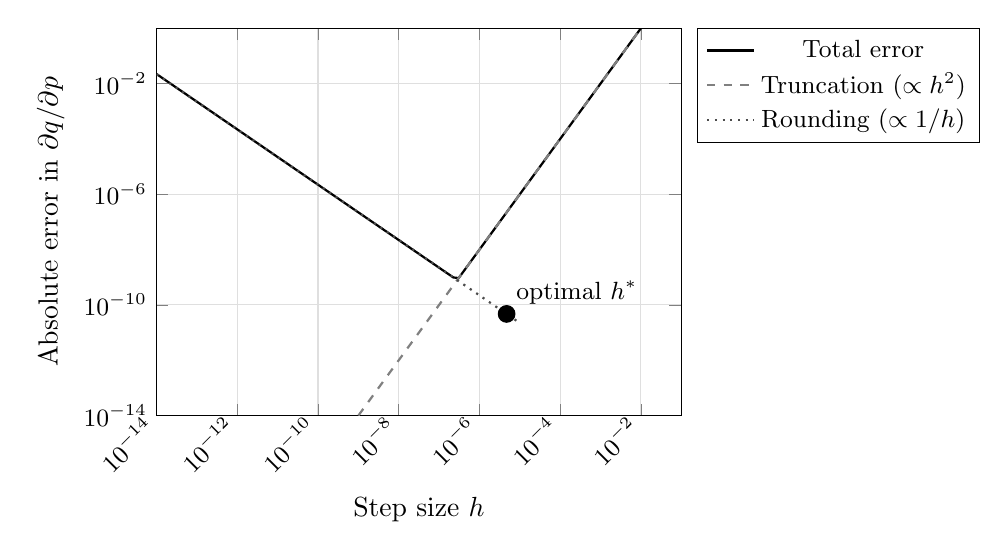
\begin{tikzpicture}
\begin{loglogaxis}[
  width=0.68\textwidth,
  height=6.5cm,
  xlabel={Step size $h$},
  ylabel={Absolute error in $\partial q/\partial p$},
  xmin=1e-14, xmax=1e-1,
  ymin=1e-14, ymax=1,
  xtick={1e-14,1e-12,1e-10,1e-8,1e-6,1e-4,1e-2},
  xticklabel style={rotate=45, anchor=east, font=\small},
  ytick={1e-14,1e-10,1e-6,1e-2},
  yticklabel style={font=\small},
  grid=major,
  grid style={gray!25},
  legend pos=outer north east,
  legend style={font=\small},
]
%% Truncation error: slope -2 (centered diff)
\addplot[thick, black, domain=1e-14:1e-1, samples=100]
  {max(x^2 * 1e4, 2.2e-16 / x)};
  \addlegendentry{Total error}

%% Truncation only
\addplot[thick, dashed, black!50, domain=1e-9:1e-1, samples=50]
  {x^2 * 1e4};
  \addlegendentry{Truncation ($\propto h^2$)}

%% Rounding only
\addplot[thick, dotted, black!70, domain=1e-14:1e-5, samples=50]
  {2.2e-16 / x};
  \addlegendentry{Rounding ($\propto 1/h$)}

%% Optimal h marker
\addplot[mark=*, mark size=3pt, only marks, black]
  coordinates {(4.7e-6, 4.7e-11)};
  \node[above right, font=\small] at (axis cs:4.7e-6, 4.7e-11)
    {optimal $h^*$};
\end{loglogaxis}
\end{tikzpicture}
\caption{The U-curve for centered differences in double precision.
         Truncation error (dashed) decreases as $h$ decreases;
         rounding error (dotted) increases. The total error (solid)
         is minimized at the optimal step size $h^*$.
         Using $h$ much smaller than $h^*$: a common mistake;
         gives larger errors, not smaller ones.}
\label{fig:ucurve}
\end{figure}

Setting the two error contributions equal gives an approximate
starting point for step-size selection:
\begin{align}
  h^*_{\text{forward}}  &\approx \sqrt{\varepsilon_{\text{mach}}}\cdot|p^*|
                          \approx 1.5 \times 10^{-8}\cdot|p^*|,
  \label{eq:hopt_fwd} \\
  h^*_{\text{centered}} &\approx \varepsilon_{\text{mach}}^{1/3}\cdot|p^*|
                          \approx 6 \times 10^{-6}\cdot|p^*|.
  \label{eq:hopt_cen}
\end{align}
For a parameter with nominal value $p^* = 0.3$, this suggests
a starting centered-difference step of approximately
$h \approx 1.8 \times 10^{-6}$.

These formulas should be understood as rough guides, not precise
prescriptions. The unknown third derivative $q'''(p)$ makes
the exact truncation error inaccessible, so the
true optimal $h$ depends on the specific model being analyzed.
The practical workflow described in Section~\ref{sec:finitediff},
computing the error indicator~\eqref{eq:FDerror} and
adjusting $h$ until the one-sided and centered approximations
agree to acceptable precision, is more reliable in practice
than relying on these theoretical formulas alone.

The most common mistake in finite-difference SA is choosing $h$
that is too small. Practitioners who set $h = 10^{-12}$ or
$h = 10^{-15}$, reasoning that ``smaller is more accurate,''
obtain results dominated by catastrophic cancellation
(subtracting two nearly equal floating-point numbers, which destroys
significant digits and amplifies rounding error).
The U-curve explains why: below the optimal step size,
rounding error grows as $1/h$ while truncation error continues
to fall, so the total error increases rather than decreases.
The error indicator~\eqref{eq:FDerror} will detect this failure:
when $h$ is too small, the centered and forward approximations
both carry large rounding errors and will disagree by a large
relative amount, signaling that a larger step size is needed.

The U-curve also reveals a practical limitation for models
implemented with adaptive ODE solvers.
For a smooth analytic function the curve has a well-defined minimum,
and the error indicator~\eqref{eq:FDerror} decreases reliably as
$h$ is reduced toward the optimal step size.
For a model that calls \texttt{ode45} internally, the output is not
mathematically smooth: the solver makes discrete step-size decisions
that can cause the model output to change non-smoothly as a
parameter varies by a small amount.
In these cases the error indicator may not decrease monotonically,
and the one-sided and centered approximations may disagree by more
than machine precision even at step sizes near $10^{-6}|p^*|$.
The remedy is to tighten the ODE solver tolerances
(\texttt{RelTol} and \texttt{AbsTol} in \texttt{ode45}) before
reducing $h$ further. After tightening tolerances, applying
the adaptive workflow (compute the error indicator,
check for agreement, reduce $h$ if needed) usually
locates a reliable step size.

\begin{selfcheck}
For the SIR model with transmission probability $\beta^* = 0.06$,
the theoretical formula~\eqref{eq:hopt_cen} suggests a starting
centered-difference step of $h \approx 3.6 \times 10^{-7}$.
You then compute the centered difference and a one-sided forward
difference at this $h$ and find they agree to four significant
figures.
(a) Is this step size acceptable? What does this agreement indicate?
(b) Now suppose you repeat the check at $h = 10^{-12}$ and find the
two approximations disagree by more than 50\%. What does this signal,
and what should you do?
\end{selfcheck}
\begin{scAnswer}
(a) Agreement to four significant figures indicates that the
rounding error is small relative to the truncation error at this
$h$, and the centered approximation is reliable.
The step size is acceptable for four-digit SI accuracy.

(b) Large disagreement at $h = 10^{-12}$ signals that rounding error
dominates: both approximations suffer catastrophic cancellation.
The remedy is to increase $h$ toward the range suggested by the
theoretical formula, then recheck the error indicator.
Rounding error $\propto 1/h$: at $h = 10^{-12}$ the rounding error
is $(3.6\times10^{-7}/10^{-12}) = 3.6\times10^5$ times larger than
at $h^* \approx 3.6\times10^{-7}$. Moving to even larger $h$ would
re-introduce truncation error, so the reliable range lies in between.
\end{scAnswer}

%%------------------------------------------------------------
\section{Second-Order Terms}
\label{sec:secondordercomp}
%%------------------------------------------------------------

Chapter~2 previewed second-order terms as corrections to the first-order
SI approximation. This section shows how to compute them.

\subsection{Pure Second-Order Derivatives}

The second derivative $\partial^2 q/\partial p_i^2$ measures the
curvature of the \QOI as a function of $p_i$.
It can be estimated by reusing the three evaluations already
computed for the centered first-order difference:
\begin{equation}
  \frac{\partial^2 q}{\partial p_i^2}
  \approx \frac{q(p^*+h\vec{e}_i) - 2q(p^*) + q(p^*-h\vec{e}_i)}{h^2}.
  \label{eq:second_pure}
\end{equation}
No additional model evaluations are needed.

When the curvature is large, the first-order SI understates the
true sensitivity for larger perturbations.
Specifically, if
\[
  \left|\frac{h}{2}\,\frac{\partial^2 q/\partial p_i^2}
                   {\partial q/\partial p_i}\right| \ll 1,
\]
the linear approximation is valid for perturbations of size $h$.
If this ratio is not small, the sensitivity index provides only
a local estimate, and Chapter~9's global SA methods are needed
for a complete picture.

\unifyingidea{3} The second-order terms computed in this section
are the first quantitative correction beyond the linearization
that defines every sensitivity index in this book.
The first-order SI is valid when the model behaves approximately
linearly near the nominal parameter values.
The second-order term tells you how quickly that approximation
degrades as perturbations grow. Chapter~9 provides the full
global picture when the linearization is no longer adequate.

\subsection{Mixed Second-Order Derivatives}

The cross-derivative $\partial^2 q/\partial p_i\,\partial p_j$
measures how the sensitivity to $p_i$ changes with $p_j$.
It requires one additional model evaluation beyond those already computed:
\begin{equation}
  \frac{\partial^2 q}{\partial p_i\,\partial p_j}
  \approx \frac{q(p^*+h\vec{e}_i+h\vec{e}_j)
              - q(p^*+h\vec{e}_i)
              - q(p^*+h\vec{e}_j)
              + q(p^*)}{h^2}.
  \label{eq:second_mixed}
\end{equation}
For all $\binom{n_p}{2}$ pairs, this requires $\binom{n_p}{2}$
additional evaluations.
For $n_p = 4$, that is 6 evaluations; for $n_p = 17$
(the malaria model), it is 136.

The cross-derivative $\partial^2 q/\partial p_i\,\partial p_j$
is large when the two \POIs \emph{interact}: varying them together
is not the same as varying them separately.
Chapter~9 shows that Sobol interaction indices $S_{ij}$ are the
global, variance-based analog of these local cross-derivatives.

\begin{selfcheck}
For the SIR model with $R_0 = k\beta\tau$,
compute $\partial^2 R_0/\partial k\,\partial\beta$ analytically.
Is the cross-derivative large or small relative to the individual
first-order derivatives $\partial R_0/\partial k$ and
$\partial R_0/\partial\beta$? What does this imply about
the interaction between $k$ and $\beta$ for $R_0$?
\end{selfcheck}
\begin{scAnswer}
$\partial^2 R_0/\partial k\,\partial\beta = \tau$
(positive, since $R_0 = k\beta\tau$).

The first-order derivatives are
$\partial R_0/\partial k = \beta\tau$ and
$\partial R_0/\partial\beta = k\tau$.

The ratio $(\partial^2 R_0/\partial k\,\partial\beta) / (\partial^2 R_0/\partial k^2) = \tau / 0$
is undefined (the pure second derivative is zero for a monomial).
More informatively, the mixed partial is nonzero, meaning $k$ and $\beta$
interact in their effect on $R_0$: increasing both together increases $R_0$
more than the sum of the individual increases. This is expected because $R_0$
is multiplicative in $k$ and $\beta$.
For Sobol analysis, this interaction will produce a nonzero $S_{k\beta}$.
\end{scAnswer}

%%------------------------------------------------------------
\section{Correlated POIs --- The Most Common Mistake}
\label{sec:correlatedPOIs}
%%------------------------------------------------------------

\begin{tcolorbox}[colback=gray!8, colframe=gray!40, boxrule=0.4pt, arc=2pt]
\textit{A parameter can be uncertain without being important,
and important without being uncertain.
Correlation between parameters adds a third possibility:
a parameter can appear important in isolation
while its true effect is inseparable from another.}
\end{tcolorbox}

\medskip

Before computing any sensitivity indices, there is a question
that must be asked: can these parameters actually be varied
independently? In many models, the answer is no.

Every finite-difference SA computation implicitly assumes that
each \POI can be perturbed while all others are held exactly fixed.
If the \POIs are correlated, meaning that in the real world,
changing one tends to change another, then this assumption
is violated and the resulting sensitivity indices can be misleading.

\subsection{Diagnosing Correlation}

Correlation among \POIs arises from several sources.

\textbf{Structural correlation}\index{correlated POIs!structural}\index{structural identifiability} occurs when parameters appear
only as a product or ratio in the model equations.
In the SIR model, the force of infection is
$\lambda = k\beta I/N$.
The parameters $k$ and $\beta$ appear only as the product $k\beta$.
Observational data, incidence counts over time, can identify
$k\beta$ as a unit but cannot separate the two factors.
Computing $\SI{k}{R_0}$ and $\SI{\beta}{R_0}$ as independent indices
is mathematically valid but can be operationally misleading,
because any intervention must target the product $k\beta$
(by reducing contact rate, transmission probability, or both).
Reparameterizing to use $k\beta$ as a single \POI is more
natural in this case.

This observation is the starting point for \textbf{structural identifiability}%
\index{structural identifiability}
\label{sec:structural_identifiability}%
analysis: the question of whether the parameters of a model can, in
principle, be recovered from the observable outputs, regardless of
measurement noise or sample size.
A model is \emph{structurally identifiable} in a parameter $p$ if distinct
values of $p$ produce distinct output trajectories.
The SIR model is not structurally identifiable in $(k, \beta)$ separately,
but is identifiable in the product $k\beta$.
Sensitivity analysis reveals this: when two parameters always have the
same sensitivity index (here $\SI{k}{q} = \SI{\beta}{q}$ for any QOI $q$),
they are structurally correlated and the model cannot distinguish them.
A sensitivity index of zero for a parameter is a related signal: the
model output does not respond to that parameter at all, which may indicate
that the parameter cannot be estimated from data.
Chapter~9 returns to identifiability in the context of global SA,
where variance-based methods provide computational tools for
detecting structural correlation across the full parameter range.
A full treatment of structural and practical identifiability, including
formal algebraic methods, is beyond the scope of this book;
see Smith~\cite{smith2014uncertainty} \S9.3 and the references therein.

\textbf{Empirical correlation}\index{correlated POIs!empirical} occurs when parameter values
are estimated from data that naturally links them.
In the malaria model studied by Chitnis, Hyman \& Cushing~\cite{chitnis2008determining},
the mosquito biting rate $\sigma_v$ and the human biting saturation
$\sigma_h$ both appear in the force of infection and are often
positively correlated across field studies.
The paper introduces the composite parameter
$\zeta = \sigma_v\sigma_h/(\sigma_v N_v^* + \sigma_h N_h^*)$
precisely to address this correlation.

\textbf{Constraint correlation}\index{correlated POIs!constraint} occurs when a physical or
biological requirement links parameters.
In models where stage durations must sum to a total
lifecycle, or where transition probabilities must sum to one,
no parameter can change without forcing compensating changes
in others.

\subsection{The Impact of Ignoring Correlation}

To see concretely what goes wrong, consider a model whose \QOI is
$q = p_1 + p_2$ where the two \POIs satisfy $p_2 = 2p_1$
(a linear constraint). The standard sensitivity indices are:
\[
  \SI{p_1}{q} = \frac{p_1}{q}\cdot 1 = \frac{p_1}{3p_1} = \frac{1}{3},
  \qquad
  \SI{p_2}{q} = \frac{p_2}{q}\cdot 1 = \frac{2p_1}{3p_1} = \frac{2}{3}.
\]
These look reasonable: the second parameter is twice as important
as the first. But in reality, $p_1$ and $p_2$ cannot be varied
independently. Any change to $p_1$ forces a change to $p_2 = 2p_1$.
The total effect of a $1\%$ increase in $p_1$ is:
\[
  \Delta q = \frac{\partial q}{\partial p_1}\,\delta p_1
           + \frac{\partial q}{\partial p_2}\,\delta p_2
           = 1\cdot(0.01p_1) + 1\cdot(0.02p_1) = 0.03p_1.
\]
The normalized total-derivative SI for $p_1$ is then
$(p_1/q)\cdot(0.03p_1/0.01p_1) = (1/3)\cdot 3 = 1$, not $1/3$.
The standard index understates the true sensitivity by a factor of three.

\subsection{Four Practical Responses}

\textbf{Response 1: Diagnose first.}
Before any SA computation, examine the correlation structure
of the \POIs. Compute the Pearson correlation matrix from any
available data on parameter values across studies or populations.
Plot scatter matrices (\texttt{plotmatrix} in MATLAB).
A correlation $|\rho_{ij}| > 0.5$ warrants attention.

\textbf{Response 2: Reparameterize structurally correlated pairs.}
When two parameters appear only as a product or ratio,
define that product or ratio as the natural \POI.
For the SIR model: use $k\beta$ as a single \POI, with
the composite sensitivity index
$S_{k\beta}^{R_0} = \SI{k}{R_0} + \SI{\beta}{R_0} = 1 + 1 = 2$.
(The additive rule for sensitivity of composite parameters
is developed in the exercises.)

\textbf{Response 3: Total derivative for empirically correlated pairs.}
When empirical data establishes that a proportional change in $p_i$
induces a proportional change in $p_j$ with coefficient $c_{ij}$
(i.e., $\Delta p_j/p_j \approx c_{ij}\,\Delta p_i/p_i$),
the total derivative SI is:
\begin{equation}
  \SI{p_i}{q}\big|_{\mathrm{tot}}
  = \SI{p_i}{q}\big|_{\mathrm{std}}
  + \sum_{j \neq i} \SI{p_j}{q}\,c_{ij}.
  \label{eq:totalSI}
\end{equation}
In plain language: $c_{ij}$ is the induced proportional change in $p_j$
per unit proportional change in $p_i$. If a $1\%$ increase in $k$
tends to be accompanied by a $0.6\%$ increase in $\beta$ (from field data),
then $c_{k\beta} = 0.6$. Estimate $c_{ij}$ from regression of observed
parameter pairs, or from domain knowledge about shared drivers.
Report both the standard and total-derivative SIs together with
the correlation coefficients so readers can assess the impact.

\textit{Response 4} (Report transparently).
When correlations exist but cannot be fully quantified,
state explicitly in the SA report that the independence
assumption was made, identify the correlated pairs,
and flag which SI values are most likely affected.

\begin{selfcheck}
In the SIR model, the product $k\beta$ represents the effective
transmission rate. If a field study establishes that $k$ and $\beta$
are positively correlated with coefficient $c_{k\beta} = 0.4$
(i.e., $\Delta\beta \approx 0.4\,\Delta k$ for proportional changes),
use equation~\eqref{eq:totalSI} to compute the total-derivative SI
of $R_0$ with respect to $k$ at the nominal values.
Compare with the standard SI $\SI{k}{R_0} = 1$.
\end{selfcheck}
\begin{scAnswer}
$\SI{k}{R_0} = 1$, $\SI{\beta}{R_0} = 1$.
Here $c_{k\beta} = 0.4$ means $(\Delta\beta/\beta)/(\Delta k/k) = 0.4$,
so $p_\beta c_{k\beta}/p_k = \beta\cdot 0.4/k$.
But in proportional terms: total SI $\approx 1 + 1 \times 0.4 = 1.4$.
A $1\%$ increase in $k$ (with the correlated $0.4\%$ increase in $\beta$
it entails) increases $R_0$ by approximately $1.4\%$, not $1\%$.
The standard SI underestimates the true effect by $40\%$.
\end{scAnswer}

%%------------------------------------------------------------
\section{Black-Box Models and the MATLAB Template}
\label{sec:blackbox}
%%------------------------------------------------------------

When the model is inherited code, a compiled simulation,
or a package you did not write, analytical differentiation is
not possible. Finite differences are then the only option for
local SA, and they work for \emph{any} model that accepts a
parameter vector and returns a \QOI vector.

Students sometimes treat finite differences as an inferior
approximation to be used only when analytic derivatives are
unavailable. For black-box models, this framing is backwards:
finite differences are not a fallback; they are the correct and
complete tool. The accuracy they provide at the optimal step size
is typically more than sufficient for SA decisions, and their
applicability to models of arbitrary complexity makes them
indispensable in practice.

The following MATLAB function computes the full normalized
sensitivity Jacobian by centered differences, using the optimal
step size from~\eqref{eq:hopt_cen}.
Students should copy this template for every black-box SA problem.

\begin{small}
\begin{verbatim}
%% From: src/core/sensitivity_jacobian.m (see GitHub repository)
p     = sir_nominal();
R0_fn = @(pv) pv(1)*pv(2)*pv(3);   %% R0 = k*beta*tau
p_vec = [p.k; p.beta; p.tau; p.L];
[S, info] = sensitivity_jacobian(R0_fn, p_vec, 1);
%% S(j) = SI_{p_j}^{R0};  info.n_evals = 2*n_p+1 = 9

%% If n_q is wrong, the function catches it immediately:
%% >> sensitivity_jacobian(R0_fn, p_vec, 3)
%% Error: MODEL returned 1 value but N_Q = 3.
\end{verbatim}
\end{small}

The function handles the near-zero \QOI case using the regularized
change from Chapter~2. The \texttt{max} in the step-size formula
prevents $h$ from being identically zero when $p_{\text{nom},i} = 0$.

To validate this template on any model, call it with the analytic
sensitivity indices known from Chapter~2 and verify agreement.
For the SIR model:

\begin{verbatim}
%% SIR R0 as function of p = [k, beta, tau]
R0_model = @(p) p(1)*p(2)*p(3);    %% R0 = k * beta * tau

p_nom = [5, 0.06, 7];     %% nominal: k, beta, tau
S = sensitivity_jacobian(R0_model, p_nom, 1);

fprintf('Sensitivity indices for R0:\n')
fprintf('  SI_k    = %6.4f  (exact: 1.0000)\n', S(1))
fprintf('  SI_beta = %6.4f  (exact: 1.0000)\n', S(2))
fprintf('  SI_tau  = %6.4f  (exact: 1.0000)\n', S(3))
\end{verbatim}

\begin{selfcheck}
The template above uses $h_{\min} = 10^{-10}$ as a floor for the
step size. Why is this floor necessary, and what happens if a
\POI has nominal value exactly zero?
\end{selfcheck}
\begin{scAnswer}
If $p_{\text{nom},i} = 0$, then $6 \times 10^{-6}|p_{\text{nom},i}| = 0$,
giving $h = 0$ and a division-by-zero error.
The floor $h_{\min} = 10^{-10}$ prevents this.
For a \POI with nominal value zero, the step size is not scaled
by the parameter magnitude, it is just the fixed small value $10^{-10}$.
In this case, the SI is also not well-defined in the ratio form
(it would require dividing by $p_i = 0$), so the code computes
the unnormalized derivative instead.
If a \POI is exactly zero at its nominal value, the
investigator should either reparameterize or report the
absolute (unnormalized) derivative rather than the normalized SI.
\end{scAnswer}

%%------------------------------------------------------------
\section[MATLAB Laboratory]{MATLAB Laboratory: SA of the SIR Model by Finite Differences}
\label{sec:ch3matlab}
%%------------------------------------------------------------

This laboratory puts the chapter's tools together and provides
a complete reference implementation for black-box SA.
Use the SIR ODE model with the four \POIs $\{k, \beta, \tau, \mu\}$
and the three \QOIs $\{S(T), I(T), R(T)\}$ at time $T = 60$~days.

\textbf{Setup.}
Implement \texttt{SIR\_model(p)} as a MATLAB function that takes
the parameter vector $p = [k, \beta, \tau, \mu]$ and returns
$[S(60), I(60), R(60)]$ by calling \texttt{ode45}.
Use nominal values $k = 5$, $\beta = 0.06$, $\tau = 7$~days,
$\mu = 0.0001$~day$^{-1}$, and initial conditions
$S_0 = 999$, $I_0 = 1$, $R_0 = 0$.

\textbf{Part 1:} Compute the full sensitivity Jacobian.
Call \texttt{sensitivity\_jacobian(SIR\_model, p\_nom, 3)}
to produce the $3 \times 4$ sensitivity matrix.
Display it as a labeled table with \QOI names as row labels
and \POI names as column labels.

\textbf{Part 2:} Plot the U-curve.
Fix all parameters at nominal values except $\beta$.
Estimate $\partial I(60)/\partial\beta$ using centered differences
for $h = 10^{-1}, 10^{-3}, 10^{-5}, 10^{-7}, 10^{-9}, 10^{-11}, 10^{-13}$.
Compute the absolute error using the fourth-order formula~\eqref{eq:FD4}
as a reference value (computed at $h = 10^{-4}$ where it is accurate).
Also plot the one-sided forward difference error at each $h$.
Plot centered-difference error, forward-difference error, and the
discrepancy between the two (the practical error indicator~\eqref{eq:FDerror})
vs.\ $h$ on log-log axes. Identify the range of $h$ where the
error indicator is small and the centered approximation is reliable.

\textbf{Part 3:} Tornado plots.
Using the Jacobian from Part~1, produce separate tornado plots
for each \QOI: the sensitivity of $S(60)$, $I(60)$, and $R(60)$
with respect to all four \POIs. Interpret: which \POI matters
most for each \QOI? Do the three plots give the same ranking?

\textbf{Part 4:} Correlation check.
The contact rate $k$ and transmission probability $\beta$
appear only as the product $k\beta$ in the SIR force of infection.
Confirm numerically that $\SI{k}{I(60)} \approx \SI{\beta}{I(60)}$
at the nominal values. Then reparameterize: define a new \POI
$\lambda_0 = k\beta$ and compute $\SI{\lambda_0}{I(60)}$.
Verify that $\SI{\lambda_0}{I(60)} = \SI{k}{I(60)} + \SI{\beta}{I(60)}$.

\textbf{Part 5:} Correlation check from literature.
The SIR force of infection is $\lambda = k\beta I/N$, so $k$ and $\beta$
appear only as the product $k\beta$ and are structurally correlated.
Use the four-parameter SIR model. Confirm numerically that
$\SI{k}{I(60)} \approx \SI{\beta}{I(60)}$ at nominal values.
Then search the epidemiological literature for any reported correlations
between contact rates $k$ and transmission probabilities $\beta$
across outbreak settings.
Construct a $4\times4$ correlation matrix using whatever estimates you find,
or assume a moderate positive correlation $\rho_{k\beta} = 0.6$
and zero for all other pairs.
Use equation~(3.6) to compute the total-derivative SI of $I(60)$
with respect to $k$ accounting for this correlation.
Compare with the standard SI and discuss the practical difference.

\textbf{Extension.}
Using equation~\eqref{eq:second_pure}, compute the pure second-order
sensitivities $\partial^2 I(60)/\partial p_i^2$ for each of the
four \POIs. For each parameter, assess whether the second-order
term is large enough to matter for $10\%$ perturbations.
(Reuse evaluations from Part~1 to keep the additional cost minimal.)

%%------------------------------------------------------------
\section{Exercises}
\label{sec:ch3exercises}
%%------------------------------------------------------------

\begin{exercise}[\bloom{L2}]
\label{ex:ch3:ucurve}
Explain in your own words why making the step size $h$ smaller
does not always improve the accuracy of a finite-difference
sensitivity estimate. Describe the two sources of error and
explain why they act in opposite directions as $h$ changes.
\end{exercise}

\begin{exercise}[\bloom{L3}]
\label{ex:ch3:cost}
A model has $n_p = 15$ \POIs and $n_q = 4$ \QOIs.
\begin{enumerate}[label=(\alph*)]
  \item Fill in Table~\ref{tab:FDcost} for this model:
        how many model evaluations does each method require?
  \item If each evaluation takes 30~seconds,
        how long does the centered-difference Jacobian take?
  \item At what point (in terms of $n_p$ and evaluation time)
        would the adjoint method from Chapter~6 be strictly necessary?
\end{enumerate}
\end{exercise}

\begin{exercise}[\bloom{L3}]
\label{ex:ch3:ucurve_matlab}
For the function $q(p) = \sin(p^2)$ at $p^* = 1.3$,
compute $\partial q/\partial p$ using centered differences
for $h \in \{10^{-1}, 10^{-2}, \ldots, 10^{-14}\}$.
Compare each estimate to the exact value $q'(p) = 2p\cos(p^2)$.
Plot error vs.\ $h$ on log-log axes and identify the optimal $h$.
Does it agree with the formula in equation~\eqref{eq:hopt_cen}?
\end{exercise}

\begin{exercise}[\bloom{L3}]
\label{ex:ch3:second}
For the SIR model $R_0 = k\beta\tau$:
\begin{enumerate}[label=(\alph*)]
  \item Compute the pure second derivatives $\partial^2 R_0/\partial k^2$,
        $\partial^2 R_0/\partial\beta^2$, $\partial^2 R_0/\partial\tau^2$
        analytically. What do you notice?
  \item Compute the cross derivatives $\partial^2 R_0/\partial k\,\partial\beta$,
        $\partial^2 R_0/\partial k\,\partial\tau$,
        $\partial^2 R_0/\partial\beta\,\partial\tau$ analytically.
  \item For a $10\%$ perturbation to $k$ and a simultaneous $10\%$ perturbation
        to $\beta$, estimate the true change in $R_0$ using both the
        first-order and the full second-order Taylor approximations.
        How large is the correction?
\end{enumerate}
\end{exercise}

\begin{exercise}[\bloom{L4}]
\label{ex:ch3:correlatedSIR}
In the SIR model, suppose field data suggests that the
contact rate $k$ and transmission probability $\beta$ are
positively correlated: across outbreak settings,
when $k$ increases by $10\%$, $\beta$ tends to increase by $6\%$.
\begin{enumerate}[label=(\alph*)]
  \item Compute the standard sensitivity indices $\SI{k}{R_0}$
        and $\SI{\beta}{R_0}$.
  \item Using equation~\eqref{eq:totalSI}, compute the total-derivative
        SI of $R_0$ with respect to $k$, accounting for the correlation.
  \item Which is larger: the standard SI or the total-derivative SI?
        What does this mean for a policy maker who can reduce
        contact rates (through social distancing) but not transmission
        probability directly?
\end{enumerate}
\end{exercise}

\begin{exercise}[\bloom{L4}]
\label{ex:ch3:blackbox}
A colleague provides you with the function \texttt{seir\_model(p)}
that implements a SEIR epidemic model with $n_p = 6$ parameters
and returns the peak infection count as a single \QOI.
Each model evaluation takes approximately 0.2~seconds.
\begin{enumerate}[label=(\alph*)]
  \item How long will it take to compute the complete sensitivity
        Jacobian using centered differences?
  \item Apply the \texttt{sensitivity\_jacobian} template to this model.
        What additional information do you need before interpreting
        the results? (Think about parameterization.)
  \item You find that two of the six parameters have
        $|\rho_{ij}| = 0.78$. What should you do before
        reporting the sensitivity indices?
\end{enumerate}
\end{exercise}

\begin{exercise}[\bloom{L5}]
\label{ex:ch3:studydesign}
A government agency funds you to perform SA on a dengue fever
transmission model with 9 parameters and 3 \QOIs
(peak infections, total deaths, days until outbreak peak).
Each model evaluation takes 4~minutes.

Design the complete computational SA study.
Your design should specify:
\begin{enumerate}[label=(\alph*)]
  \item Which finite-difference method you will use and why.
  \item The total computation time.
  \item How you will choose the step size for each parameter.
  \item What checks you will run before reporting any results.
  \item How you will present the results to a non-technical audience.
  \item One scenario in which the standard SA would give misleading
        results, and what you would do instead.
\end{enumerate}
\end{exercise}

\begin{exercise}[\bloom{L6}]
\label{ex:ch3:critique}
A published sensitivity analysis reports:
``All finite-difference computations used $h = 10^{-12}$
to ensure maximum precision. The code was run in MATLAB
using double-precision arithmetic.''

The authors report that for several parameters, the sensitivity
indices are exactly zero to all reported decimal places.

Identify what is most likely wrong with these results
and explain your reasoning quantitatively, using the
U-curve analysis from Section~\ref{sec:ucurve}.
What should the authors have done, and how would you
determine whether the zero SI values are genuine or numerical artifacts?
\end{exercise}

%%------------------------------------------------------------

